A time-travelling secret agent arrives at Kurt Gödel’s apartment in the middle of a night in 1929 to retrieve a mobile phone that her colleague had left behind while taking a selfie. The mission is of vital importance, as if she fails, the fabric of space-time will be profoundly damaged. The colleague left her a detailed plan of the house, specifying which doors he has left unlocked, and told her where the phone is located. Our agent must navigate through the house, possibly unlocking any locked doors and retrieve the lost mobile phone. If there is already an unlocked door between two rooms, she may simply pass. She may unlock any locked door if she is in one of the two rooms connected by it. As she is interested in doing this before the brilliant mind awakes, she needs to make as few moves as possible. 

\begin{enumerate}[label=(\alph*)]
    \item  Design two STRIPS actions, one for crossing from one room to another and one for unlocking a locked door between two rooms. Define the variables to model different aspects of this exercise on your own and describe them in detail.
    \item You are given the blueprint of the house that the agent received. Rooms are lebeld with $r_1,\ldots ,r_7$. Thick lines on the walls indicate a door between two rooms and are labeled with $d_1,\ldots ,d_9$. The agent was told that the doors $d_2,d_5$ and $d_9$ have been left unlocked. Upon arriving in the alternate timeline, she finds herself in the room $r_1$ while the phone is in the room $r_7$. Formulate the initial state of the given planning setting and use \textit{progression planning} to find a plan to retrieve the phone. What do the goal states look like?
\end{enumerate}

\begin{figure}[h!]
    \centering
    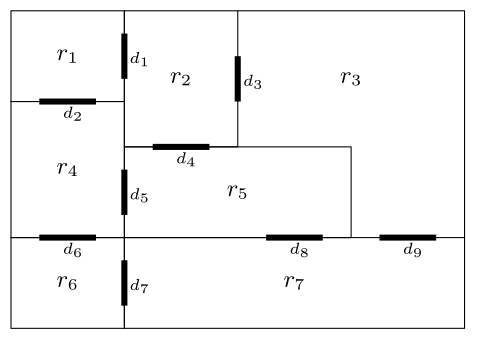
\includegraphics[scale=0.5]{img/room.png}
\end{figure}

